\documentclass[10pt, a4paper]{article}
\usepackage[T2A]{fontenc}
\usepackage[utf8]{inputenc}
\usepackage[english, russian]{babel}
\usepackage[OT1]{fontenc}
\usepackage{amsmath}
\usepackage{amsfonts}
\usepackage{amssymb}
\usepackage[version=4]{mhchem}
\usepackage{stmaryrd, caption}
\usepackage{graphicx}
\usepackage{chemfig}
\setchemfig{
  atom sep=14.4pt,
  double bond sep=2.6pt,
  bond style={line width=0.6pt},
  cram width=2.0pt,
  angle increment=60
}
\renewcommand*\printatom[1]{\small\ensuremath{\mathsf{#1}}}
\usepackage[margin=30pt]{geometry}
\usepackage[export]{adjustbox}
\graphicspath{{./pics}}

\title{Перевод статьи ``Core-Shell Magnetite-Gold Nanoparticles: Preparing and Functionalization by Chymotrypsin"}


\author{Демурин Артём Андреевич \\ Гук Ярослав Андреевич  \\ Веселов Сергей Вячеславович}
\date{}


\DeclareUnicodeCharacter{0131}{\ifmmode\imath\else{$\imath$}\fi}

\begin{document}
\maketitle

\begin{abstract}
В данной работе мы представляем результаты синтеза наночастиц (МНЧ) магнетита-
золота типа ядро-оболочка. Подготовка наночастиц состоит из нескольких стадий:
синтез ядра (Из магнетита. --- прим. студ), его покрытие золотой обочлочкой,
очищение частиц магнетита-золота (``from an uncoated magnetite'' из оригинальной
статьи немного сбивает с толку, имеется ввиду очищение от без-оболочных частиц
магнетита. --- прим. студ), и функционализация действием серосодержащих лиганд.
Условия, нужные для функционализации наночастиц липоевой кислотой и меркапто-метокси
полиэтилен гликолем (в тексте $\text{HSPEGOCH}_3$. --- прим. студ), детально описаны,
что позволяет определять оптимальные условия для эффективного очищения и 
максимальной концентрации частиц в растворе для применения в биологических 
тестах. Возможность дистанционно влиять на свойства химотрипсина было продемонстрированно
на примере его смеси с раствором наночастиц магнетита-золота. Наночастицы
магнетита-золота полученные нами обещяют многое для будущего применения 
в биомедицине.
\end{abstract}

\section*{ВВЕДЕНИЕ}
В последнее десятилетие наночастицы оксидов железа получили широкое распространение в биомедицинских исследованиях. В ряде публикаций,
магнитные наночастицы предлагается использовать в лечении онкологических патологий с применением гипертермического метода,
транспорта и адресной доставки лекарств для получения опухолеселективных МРТ-контрастных агентов [1-5]. Были предприняты попытки использования магнитных наночастиц
в качестве агентов-медиаторов для дистанционного управления биохимическими реакциями [6]. Магнитные наночастицы являются перспективными благодаря
благодаря их сильным магнитным свойствам [7-9], но они обладают рядом недостатков: склонность к быстрой агрегации в
растворе, сложность функционализации и токсичность. Покрытие магнитных наночастиц неорганической оболочкой, например, золотом,
позволяет устранить указанные недостатки.

Целью данной работы являлся синтез и физико-химическое изучение систем на основе наночастиц магнетита (МНЧ)
с заданными свойствами для биомедицинского применения и изучение возможности влияния переменного магнитного поля
на биомолекулы, иммобилизованные на поверхности МНЧ. Для устранения перечисленных недостатков мы использовали покрытие
МНЧ золотом, которое стабилизирует их, снижает токсичность частиц до минимума и позволяет модифицировать
наночастицы широким спектром серосодержащих лигандов, что, в свою очередь, упрощает модификацию поверхности [10].

На сегодняшний день существует множество работ, посвященных покрытию МНЧ золотой оболочкой [11-13], однако проблема
оптимизации метода синтеза таких частиц остается актуальной из-за большого различия в природе поверхности магнетита и золота и соответствующей необходимостью проведения стадии очистки. 
В связи с этим основной задачей данного исследования стало проведение очистки магнетитно-золотых частиц от частиц магнетита и проведение комплексного
физико-химического исследования наночастиц магнетит-золото.

Следующим этапом работы стала функционализация поверхности магнитных наночастиц серосодержащими органическими
лигандами, модификация с химотрипсином - ферментом, каталитические свойства которого подробно изучены в литературе, и
последующая демонстрация возможности применения магнетит-золото-белковых частиц в биомедицине. Химотрипсин был
использован в качестве модели для изучения механохимического действия переменного магнитного поля, а именно возможности регулировать
каталитическую эффективность фермента, иммобилизованного на магнитных наночастицах, за счет изменения его конформации под
действием сил поля.

Актуаьность работы заключается в оптимизации методики приготовления и очистки магнетит-золотых наночастиц и в исследовании нетермического механизма влияния магнитного поля на кинетику
ферментативных реакций с участием функционализированных магнитных наночастиц. Регуляция каталитической активности
фермента, иммобилизованного на магнитных наночастицах, с помощью поля может стать новым методом адресной доставки лекарств, а
Применение магнетит-золотых наночастиц в качестве контрастных агентов - инструмент для диагностики. В совокупности это открывает
путь к новым видам лекарственной тераностики

\section*{ЭКСПЕРИМЕНТАЛЬНЫЕ СВЕДЕНИЯ}
\section*{Общие Сведения}
Трансмиссионная электронная микроскопия проведена на приборе JEOL JEM-2100F/Cs/GIF (200 кВ, 0,8 А). Данные о
размеров наночастиц были получены путем ручного подсчета наночастиц в программе imageJ. Для подсчета использовали от 800 до 1000 частиц
для подсчета. Данные динамического рассеяния света (ДРС) были получены на приборе ZetasizerNano ZS (173 ◦ ) с использованием He-Ne
лазера (633 нм, 5 мВ). Анализ траекторий движения наночастиц проводился на приборе NanoSight NS500. Термогравиметрический
анализ (ТГА) проводили на дериватографе Netzsch STA 449C с масс-спектрометром QMS 403C. Для проведения
анализа использовались лиофилизированные образцы наночастиц, приготовленные по описанной выше методике. Нагрев образцов
до 1000◦C со скоростью 5◦C/мин проводили в платиновых тиглях в потоке воздуха. Метод позволяет одновременно регистрировать
кривую дифференциального термического анализа (ДТА), кривую ТГА, кривую дифференциального термогравиметрического анализа (ДТГА), а также
определять состав летучих продуктов по масс-спектру. Эксперименты в магнитном поле проводились
с использованием индуктометра «Астра-50» (ООО «Нанодиагностика», Россия) с многоуровневой системой охлаждения и системой
термостатического контроля кюветы.

\section*{Синтез Магнетитных Наночастиц Диаметром (9 \(\pm 2 \text{нм}\) )}
Синтез МНЧ был проведен по методу, описанном в литературе [15].

(Далее отрывок из указанной статьи. --- прим. студ)

\textbf{Синтез наночастиц $\text{Fe}_3\text{O}_4$.}  Водный раствор FeCl3 (4 $\text{см}^3$, 1 моль $\text{дм}^{-3}$ ) и FeCl2 (1 $\text{см}^3$, 2 моль $\text{дм}^{-3}$) в 2 моль $\text{дм}^{-3}$ HCl перемешивали и добавляли в разбавленный раствор NH3 (50 $\text{см}^3$, 0.7 моль $\text{дм}^{-3}$ ). Реакционную смесь перемешивали в течение 30 мин. Затем магнитной декантацией выделили осадок. Осадок перемешивали с разбавленной HClO4 (50 $\text{см}^3$ , 2 моль $\text{дм}^{-3}$ ) и отделяли центрифугированием. Остаток доводят до 50 $\text{см}^3$ водой DI (Деионизированной водой --- прим. студ). 

\section*{Покрытие Магнетитовых Наночастиц Золотой Оболочкой}
Синтез наночастиц магнетита-золота был выполнен в соответствии с [16, 17].

(Далее отрывок из статьи [17]. --- прим. студ)

120 мл водного раствора HAuCl4 (35 мг HAuCl4-3H2O) при беспощадном перемешивании нагревали 
под рефлюксом до состояния кипения, и 5 мл свежеприготовленной дисперсии МНЧ Fe3O4 быстро добавляли к раствору HAuCl4. 
Через 10 мин к реакционной смеси быстро добавили 5 мл цитрата натрия (80 мМ). Смесь кипятили под рефлюксом при энергичном перемешивании в течение 5 мин; затем нагрев выключали, и смесь охлаждали до комнатной температуры.

\section*{Очищение [18] и Функционализация Наночастиц Магнетита-Золота}
0.15 г Cефадекса G-100 растворили в 10 мл воды и оставили на ночь в холодильнике. Полученный
раствор заливали в пустой картридж (12 г) для колоночной хроматографии Interchim PF-50SIHP
для колоночной хроматографии Interchim PF-50SIHP с фильтром на дне. Затем сорбент промывали 20 мл 0.01 М цитратного буфера (pH = 5)
и раствор наночастиц Fe3O4@Au, стабилизированных цитрат-ионами (предварительно выдержанный в ультразвуковой ванне в течение 20 мин), был нанесен на сорбент.
на сорбент каплями по 15 мл. Затем сорбент промывали 10 мл 0.01 М цитратного буфера (pH = 5). На сайте
Полученный сорбент с нанесенными на него наночастицами Fe3O4@Au суспендировали в 10 мл DI H2O; 10 мл раствора
лигандов при перемешивании и оставляли на ночь. Затем проводили диализ полученного раствора
в DI воде с использованием пакетов SERVAPOR 44146 MWCO 12-14 kDa для диализа (3 раза на 1 л в течение 3 дней). Затем
раствор декантировали и пропускали через инжекторный фильтр Millipore Hydrophilic PES 0,22 мкм. Полученные 18 - 20 мл
раствора наночастиц хранили в холодильнике

\section*{Иммобилизация Химотрипсина на Поверхности Наночастицы Магнетита-Золота}
К 1 мл раствора наночастиц, предварительно выдержанного в ультразвуковой ванне в течение 20 мин, добавляли 0 - 0,25 мл цитратного буфера (20 мМ, pH5,9) так, чтобы суммарный объем раствора был равен 1 мл.
хранившихся в ультразвуковой ванне в течение 20 минут таким образом, чтобы суммарный объем раствора был равен 1 мл. Затем
К раствору добавляли необходимое количество свежеприготовленных водных растворов EDC и S-NHS (концентрация
сливных растворов составляли 10 мг/мл ). Оптимальные условия иммобилизации составляли 0,7 г EDC, 0,2 г S-NHS, 0,6 г
альфа-химотрипсина и 250 мкл цитратного буфера. После этого к 200 мкл водного раствора альфа-химотрипсина добавляли
(10 мг/мл). Затем полученный раствор помещали в шейкер на 2 ч при комнатной температуре. Последней стадией была
очистка от избытка несвязанного белка путем многократного центрифугирования раствора при 1000 g с применением
центробежных фильтров с отсечкой 100 кДа.

\section*{Определение Активности Альфа Химотрипсина}
Активность альфа-химотрипсина определяли с помощью субстрата SAAPPNA. Сначала 5 мкл субстрата SAAPPNA (концентрация 0.0016 мМ в смеси диоксан-ацетонитрил 1:1).
добавляли к 0.5 мл буферного раствора TRIS-HCl (pH 8.2) в кварцевой кювете (оптическая концентрация 0.0016 мМ).
в кварцевую кювету (длина оптического пути 1 см). Затем к раствору добавили необходимое количество раствора, содержащего альфахимотрипсин (чтобы конечная активность составляла 0.0005 - 0.005 опт. ед. / мин). После интенсивного перемешивания кювету
помещали в спектрофотометр, в котором регистрировали оптическую плотность во времени при длине волны 380 нм. Ферментативную
активность определяли по наклону полученной зависимости.\\
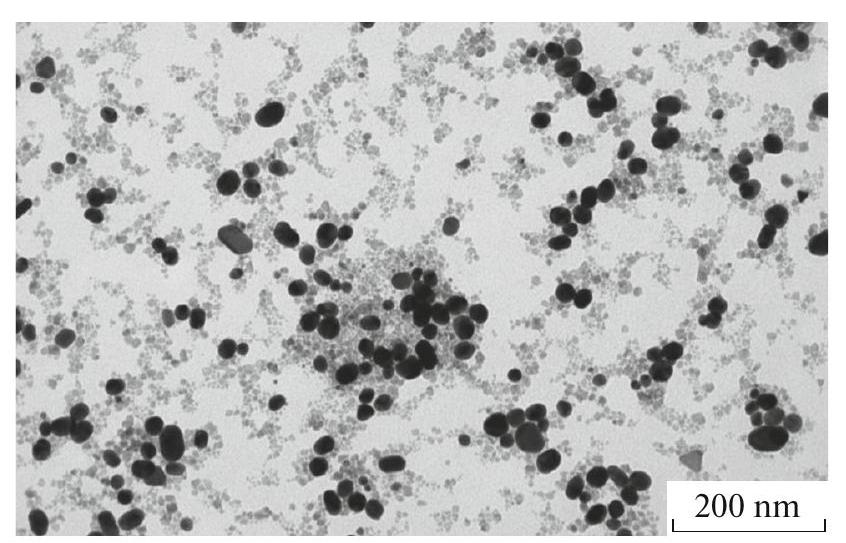
\includegraphics[scale=0.35, center]{2024_10_23_dfdc0589534473f41785g-3(1)}

Рис. 1. Наночастицы магнетита-золота под трансмиссионным электронным микроскопом.

\section*{Определение Остаточной Активности Протеинов}
Необходимое количество наночастиц с иммобилизованным ферментом в цитратном буфере (20 - 200 мкл, для получения конечной активности
0,001 - 0,005 опт. ед. /мин) добавляли в 1 мл буфера TRIS-HCl (pH 8,2). Затем содержимое интенсивно перемешивали
и распределяли по двум одинаковым светопрозрачным кюветам. Одна из кювет была контрольной; 5 мкл субстрата SAAPPNA
(концентрация 0,0016 мМ в смеси 1 : 1 диоксанa и ацетонитрила), содержимое интенсивно перемешивают и распределяют по кюветам.
интенсивно перемешивали, и кювету помещали в спектрофотометр. Одновременно другую кювету без подложки поместили
в магнитное поле. После 12-минутного пребывания в поле в эту кювету добавили 5 мкл подложки SAAPPNA, содержимое снова интенсивно перемешали и поместили в спектрофотометр.
снова интенсивно перемешивали, а кювету помещали в спектрофотометр.
Влияние поля оценивали как отношение активности в кювете, подвергшейся воздействию поля, к активности в контрольной кювете.

\section*{ВЫВОДЫ И ОБСУЖДЕНИЕ}
Синтез наночастиц Fe3O4@Au магнетит-золото проводился в два последовательных этапа. На первом этапе, согласно методике [15], были получены МНЧ со средним размером 9 ± 2 нм. На следующем этапе [16, 17] МНЧ были покрыты
золотой оболочкой путем восстановления тетрахлораурата(III) водорода цитратом натрия, который является одновременно восстановителем и стабилизирующим лигандом. Из данных ТЭМ
(рис. 1) видно, что наночастицы магнетит-золото получены в смеси с МНЧ, что согласуется с данными из литературы [19-21].

Ранее для очистки наночастиц Fe3O4@Au от МНЧ без оболочки был предложен метод хроматографической очистки
[18]. Эффективность очистки оценивали с помощью просвечивающей электронной микроскопии. На рис. 2 представлены наночастицы магнетитного золота
наночастицы после очистки. Размер наночастиц составляет 23 ± 3 нм.

Подтверждением эффективности очистки также служили данные электронной спектроскопии в УФ- и видимой областях спектра.
областях. На рисунке 3 представлены оптические спектры наночастиц Fe3O4 до нанесения оболочки, неочищенных частиц и наночастиц
после очистки и стабилизации (образец 1). Для остальных образцов наночастиц спектр поглощения после
после очистки выглядит аналогично и имеет максимум при 531 нм. Из оптических спектров, представленных на рис. 3, видно, что для
растворов наночастиц Fe3O4, а также неочищенных и очищенных наночастиц Fe3O4@Au, что очистка наночастиц
приводит к существенному уменьшению поглощения в области < 460 нм. Это связано с тем, что в процессе
хроматографии удаляются МНЧ без оболочки.

Стадия функционализации поверхности наночастиц Fe3O4@Au сопряжена со стадией очистки. Для того чтобы стабилизировать
и функционализировать наночастицы Fe3O4@Au мы использовали две различные\\
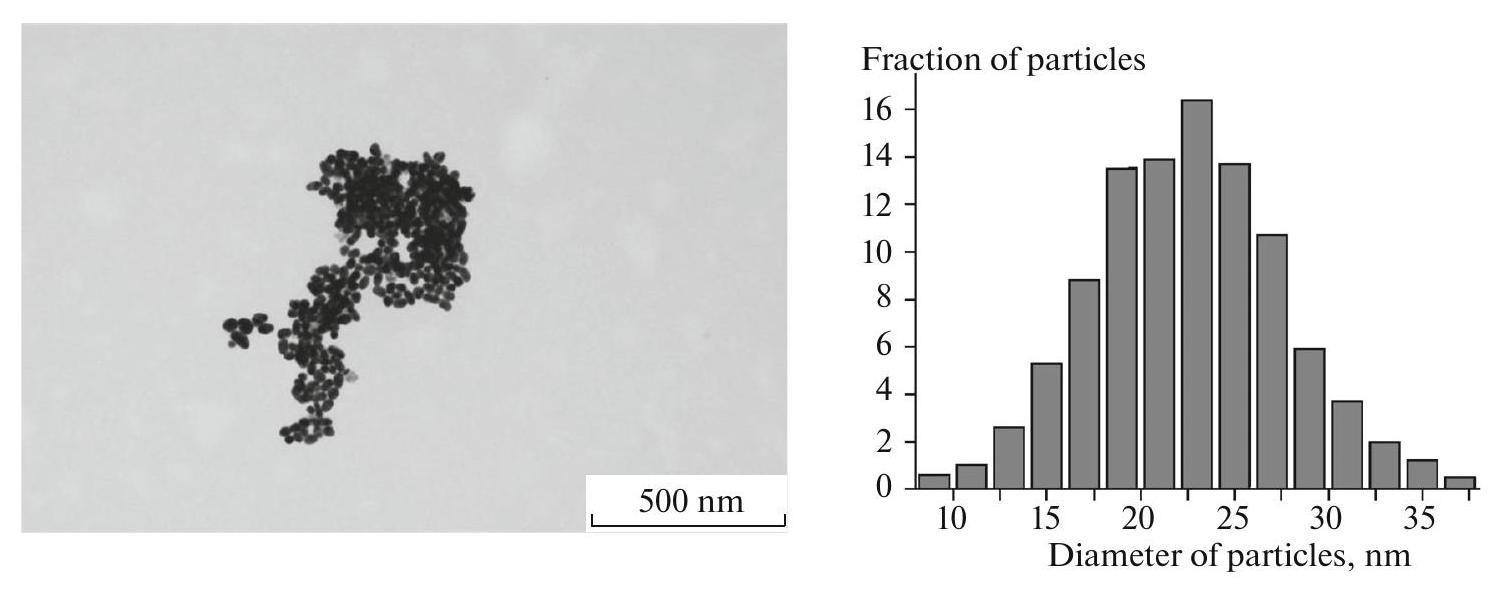
\includegraphics[scale=0.35, center]{2024_10_23_dfdc0589534473f41785g-3}

Рис. 2. Данные ТЭМ для наночастиц магнетит-золото после очистки. Гистограмма распределения по размерам.\\
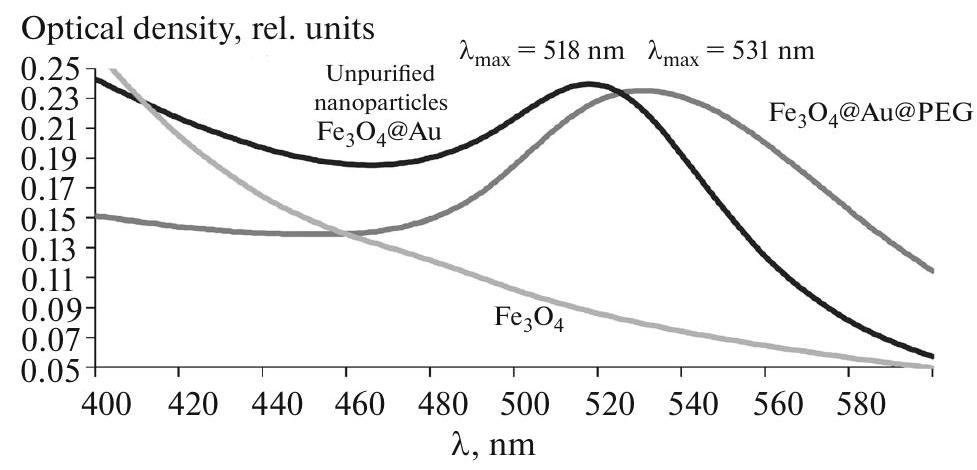
\includegraphics[scale=0.45, center]{2024_10_23_dfdc0589534473f41785g-4(1)}
Рис. 3. Спектроскопические данные в видимой области для МНЧ (светло-серый), наночастиц магнетит-золото до очистки (черный) и наночастиц магнетит-золото после очистки (серый).\\
липоевая кислота (тиоктовая кислота $C_8H_{14}O_2 S_2$) и полиэтиленгликоль (ПЭГ) с терминальной тиогруппой (HS - (CH2 - CH2 - O-)n - C, 5000 г/моль, n $\approx$ 113).
Структура лигандов представлена на рис. 4. Тиополиэтиленгликоль был выбран для того, чтобы придать коллоидную стабильность
растворов наночастиц; многие авторы проводят модификацию поверхности наночастиц с помощью подобных полимерных молекул
[22]. Для иммобилизации молекул на поверхности наночастиц необходимо использовать лиганды, содержащие функциональные
группы, например, карбоксильные или аминные; под этот критерий подходит липоевая кислота

Мы предложили использовать две лиганды в различных пропорциях для достижения, с одной стороны, стабильности коллоида и, с другой стороны, возможности иммобилизации и изучения влияния магнитного поля на фермент, иммобилизованный на поверхности наночастиц.

Для того чтобы определить количество лигандов, необходимых для модификации поверхности наночастиц, мы провели предварительную оценку максимального количества лигандов, которые могут быть размещены на поверхности наночастиц. Эта оценка была проведена на основе площади поверхности наночастицы и типичных площадей, занимаемых серосодержащими лигандами на поверхности золота. Таким образом, количество молей лиганда, которое необходимо добавить в 10 мл DI воды на последней стадии синтеза для полного покрытия поверхности наночастиц, составило \(1,03 \times 10^{-6}\) моль. Это количество удобно выражать в процентах от полного количества молей золота, добавленных на стадии очистки частиц: \(10 \%\).\\
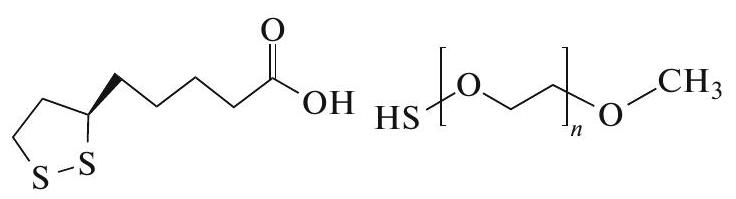
\includegraphics[scale=0.45, center]{2024_10_23_dfdc0589534473f41785g-4}

Рис. 4. Лиганды, использованные в данной работе: липоевая кислота (слева) и HSPEGOCH3 (справа).\\
В таблице приведена информация об образцах наночастиц, полученных в данной работе.

Анализ коллоидных растворов наночастиц проводился с использованием методов анализа траекторий наночастицами (NTA) и динамического рассеяния света (DLS). Анализ траекторий движения наночастиц позволяет получить информацию о концентрации образца и распределении частиц по размерам.

Полученные нами коллоидные растворы наночастиц стабильны во времени, так после 2 месяцев хранения при \(+4^{\circ} \mathrm{C}\) оптическая плотность растворов в максимуме поглощения (531 нм) составляет \(0.98-1.02\) от исходной. Концентрация наночастиц в коллоидных растворах, полученная при анализе траекторий движения наночастиц (таблица), коррелирует с оптической плотностью раствора и количеством ПЭГ, добавленного на стадии модификации поверхности наночастиц (рис. 5).

Увеличение количества \(\mathrm{HSPEGOCH}_{3}\) приводит к увеличению концентрации наночастиц в растворе. Это связано с тем, что ПЭГ облегчает удаление наночастиц с сефадекса G100 на стадии очистки. Вероятно, именно такое количество наночастиц переходит из носителя в раствор, который является коллоидно-стабильным. Поэтому добавка ПЭГ позволяет увеличить концентрацию наночастиц в коллоидном растворе.

Следует отметить, что размеры (диаметры) наночастиц, указанные в таблице, являются гидродинамическими. Кроме того, указанные в таблице размеры являются средневзвешенными значениями. Так, в случае образцов \(1-4\), средний размер, рассчитанный методом NTA, находится в диапазоне \(37-42 \text{нм}\); реальный максимум пика распределения частиц по размерам находится в диапазоне \(31-34 \text{нм}\). Эти значения вполне ожидаемы в случае частиц диаметром 23 нм, покрытых ПЭГ \((5000 \mathrm{~g} / \mathrm{mol})\) и окруженных гидратной оболочкой. Уменьшение количества ПЭГ приводит к расширению распределения частиц по размерам. Стоит отметить, что данные, полученные разными методами, согласуются друг с другом. 
Небольшая разница (в среднем больший размер

\begin{center}
\begin{table*}[h!]
\caption{Данные по всем образцам: содержание, размер и концентрация лигандов}
\scalebox{0.7}{
\begin{tabular}{c|c|c|c|c|c|c}
\hline
No. & \(\%\) of lipoic acid & \(\%\) of PEG (5000) & \begin{tabular}{c}
\(D\) (according to \\
NTA data) \\
\end{tabular} & \begin{tabular}{c}
\(D\) (according to \\
DLS data) \\
\end{tabular} & \begin{tabular}{c}
Concentration \\
(according to NTA data) \\
\end{tabular} & \begin{tabular}{c}
Optical density \\
in a peak at \(\lambda 531 \text{нм}\) \\
\end{tabular} \\
\hline
1 & 0 & 10 & 48 & 60 & \(3.7 \times 10^{11}\) & 0.814 \\
2 & 10 & 10 & 49 & 62 & \(3.0 \times 10^{11}\) & 0.732 \\
3 & 1 & \(1 / 2\) & 45 & 64 & \(2.2 \times 10^{11}\) & 0.667 \\
4 & 1 & \(1 / 4\) & 50 & 68 & \(1.2 \times 10^{11}\) & 0.348 \\
5 & 1 & \(1 / 8\) & 66 & 65 & \(8.4 \times 10^{10}\) & 0.308 \\
6 & 1 & \(1 / 16\) & 59 & 101 & \(3.0 \times 10^{10}\) & 0.122 \\
7 & 10 & 0 & 93 & 109 & \(1.5 \times 10^{10}\) & 0.066 \\
\hline
\end{tabular}}
\end{table*}
\end{center}

по данным DLS-измерений) можно объяснить тем, что методы основаны на разных физических явлениях.

Для того чтобы оценить количество лигандов, находящихся на поверхности наночастиц, мы провели термогравиметрический анализ образцов 1 и 2. Выбор именно этих образцов для анализа обусловлен возможностью использовать полученные данные для оценки максимального количества ПЭГ, которое может находиться на наночастице, проверки наличия липоевой кислоты на поверхности наночастиц и оценки ее количества. Кривые ТГА, ДТГА, дифференциальной сканирующей калориметрии (ДСК), а также ток иона с \(m / z=44 \frac{\text{г}}{\text{моль}} (\text{CO}_{2})\) представлены на рис. 6. Общая форма кривой ТГА схожа для обоих образцов: сначала происходит небольшая потеря массы образца (\(4.3 \%\) для образца 1 и \(6. 3 \%\) для образца 2 до \(200^{\circ} \mathrm{C}\) ); затем при \(235^{\circ} \mathrm{C}\) начинается довольно резкая потеря массы ( \(17. 5 \%\) для образца 1 и \(19,7 \%\) для образца 2 до \(320^{\circ} \mathrm{C}\) ), а после \(320^{\circ} \mathrm{C}\) масса
образца практически не меняется. Небольшое увеличение массы после \(400^{\circ} \mathrm{C}\) было обнаружено в случае образца 2. Пик при \(280^{\circ} \mathrm{C}\) хорошо виден на кривых ДТГА (интенсивность в максимуме составляет \(- 2 \% / \mathrm{min}\) ) для образца 1 и два пика при \(245^{\circ} \mathrm{C}\) и при \(265-270^{\circ} \mathrm{C}\) (интенсивности в максимуме составляют \(-6 \% / \mathrm{min}\) и \(-1. 5 \% / \mathrm{min}\), соответственно) для образца 2. Для обоих образцов в области \(235-320^{\circ} \mathrm{C}\), пики на кривых тока иона с \(m / z=44 \mathrm{~g} / \mathrm{mol}\left(\mathrm{CO}_{2}\right)\) и на кривых ДСК.

На основании данных [23] можно сделать вывод, что первоначальная небольшая потеря массы образцами связана с потерей воды, а существенная потеря массы при \(235-320^{\circ} \mathrm{C}\) соответствует разложению лигандов, связанных с поверхностью наночастиц. Об этом также свидетельствует увеличение ионного тока \(\mathrm{CO}_{2}\) в этой области температур. По потерям массы образца в этой области температур можно оценить количество лигандов, связанных с наночастицами.\\
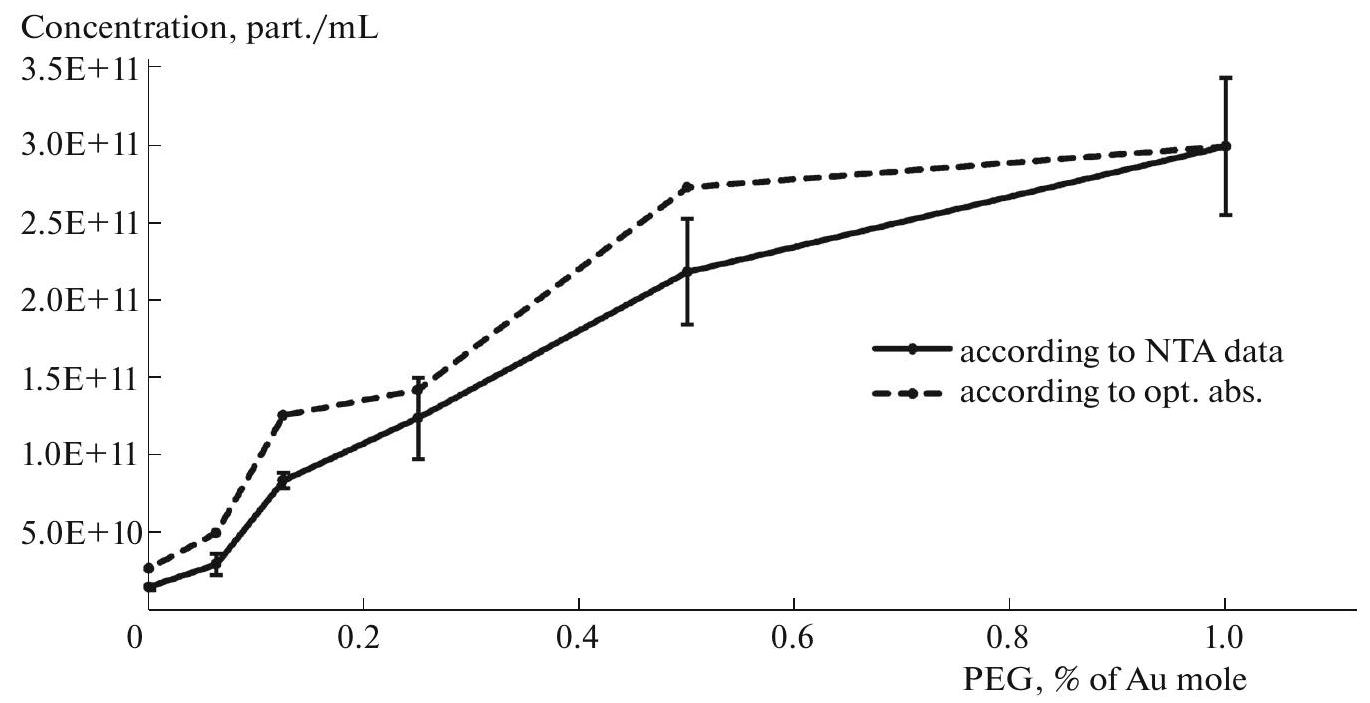
\includegraphics[scale=0.2, center]{2024_10_23_dfdc0589534473f41785g-5}
Рис. 5. Концентрации наночастиц в коллоидных растворах, полученные методом АТН и рассчитанные по оптической плотности растворов.\\
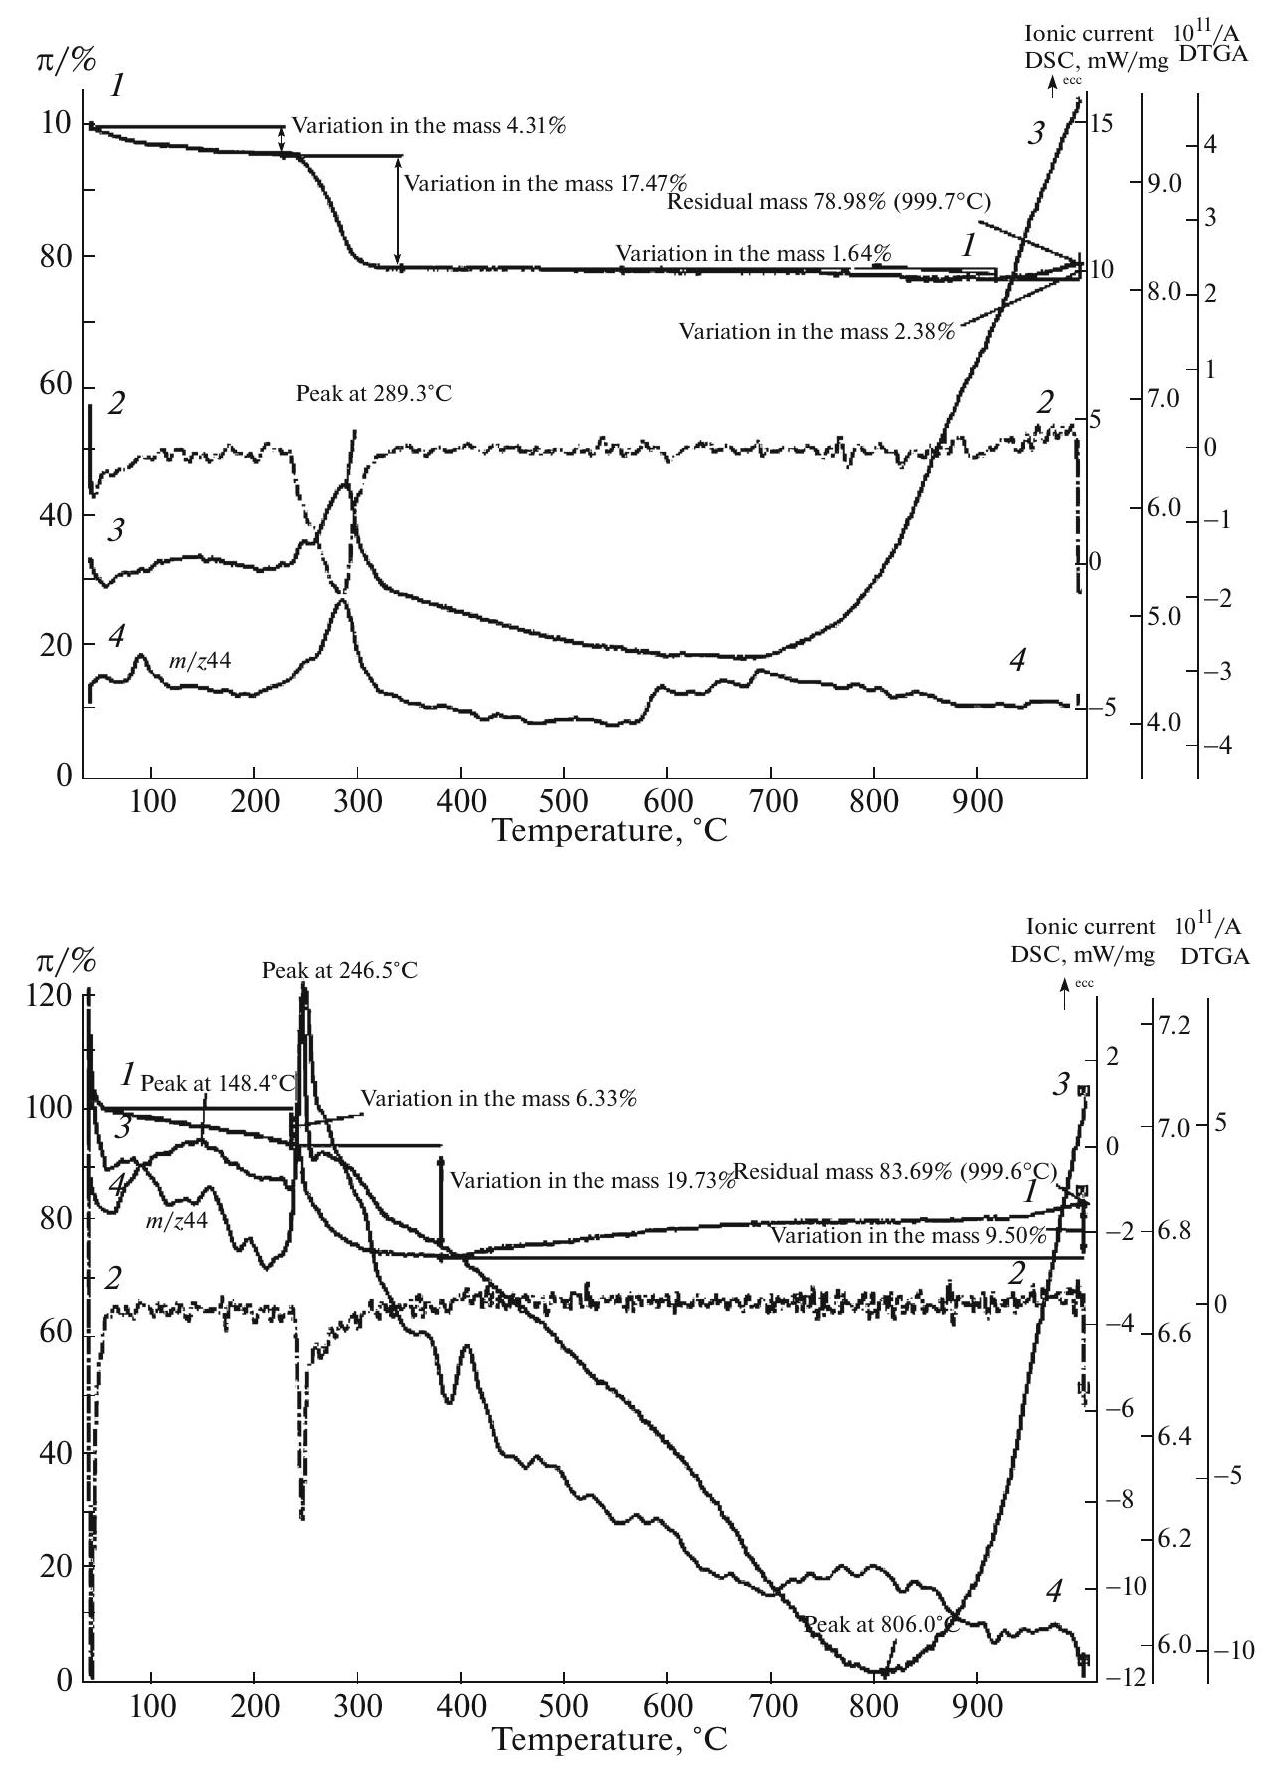
\includegraphics[scale=0.25, center]{2024_10_23_dfdc0589534473f41785g-6}
Рис. 6. Результаты термогравиметрического анализа для образцов 1 (вверху) и 2 (внизу). Потери массы по образцам: кривая ТГА (1), ее производная (2), кривая ДСК (3), кривая тока иона с \(m / z=44 \frac{\text{г}}{\text{моль}} (\text{CO}_{2})\) (4).
В случае полностью ПЭГ-лигандированного образца 1 происходит потеря \(17,5 \%\) массы. Пересчет этого значения в проценты молей золота, взятые для покрытия оболочкой 15 мл МНЧ, дает \(0,9 \pm 0,1 \%\). В случае образца 2, как было сказано выше, на кривой ДТГА можно выделить два пика. Широкий слабый пик при 265\(270^{\circ} \mathrm{C}\) может быть отнесен к процессу разложения ПЭГ (как и в случае предыдущего образца); нар-\\
рядный и более интенсивный пик при \(245^{\circ} \mathrm{C}\) может быть связан с процессом разложения липоевой кислоты. Суммарная потеря массы за счет этих процессов составляет \(19.7 \%\). Анализ профиля пиков позволяет разделить вклады обоих процессов и на основании площадей пиков сделать вывод, что потеря \(12.7 \pm 1 \%\) массы связана с разложением ПЭГ, в то время как разложение липоевой кислоты составляет\\
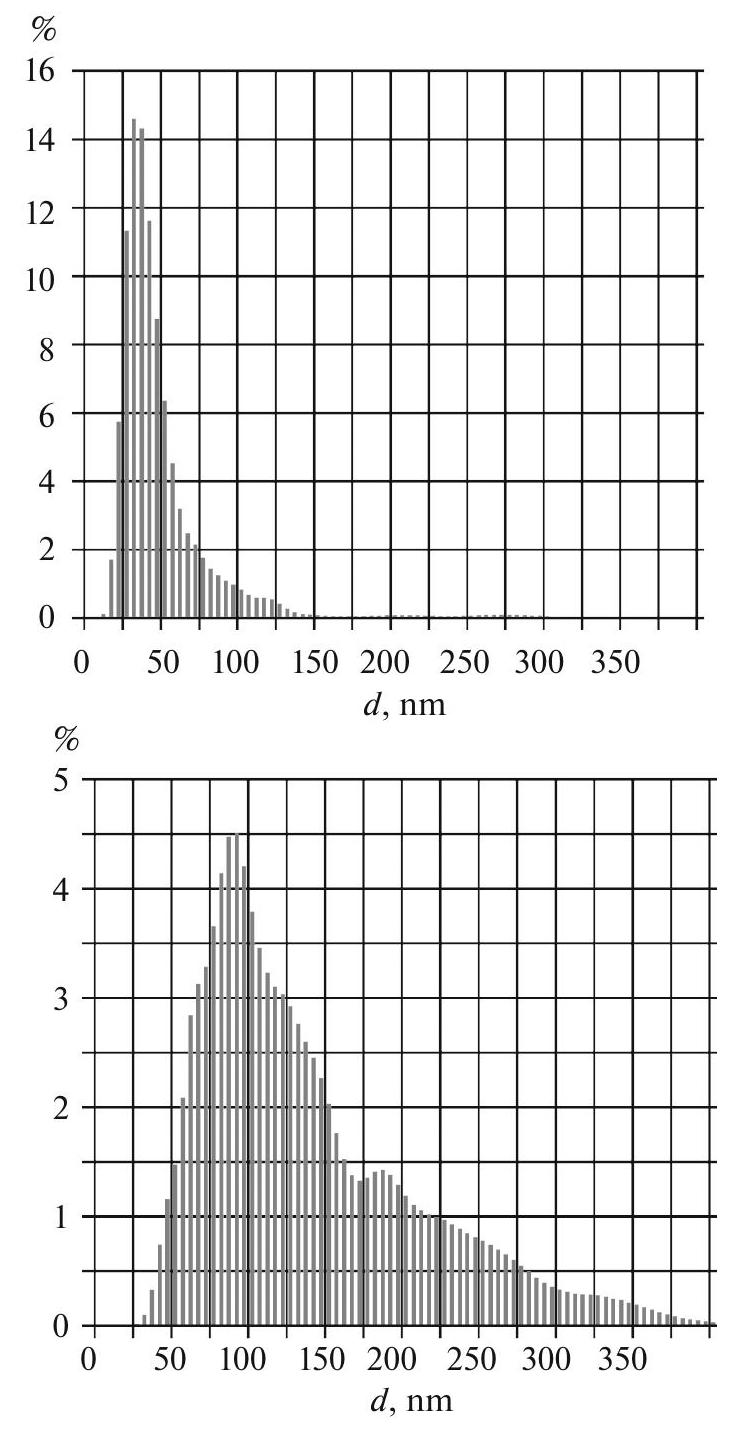
\includegraphics[scale=0.35, center]{2024_10_23_dfdc0589534473f41785g-7}
Рис. 7. Распределение частиц по размерам по данным NTA для образцов 6 (до связывания) и 8 (после связывания)\\
\(7 \pm 1 \%\) потери массы. Пересчет этих значений в проценты от молей золота дает \(1,1 \pm\)\(0,1 \%\) для ПЭГ и \(5,6 \pm 2 \%\) для липоевой кислоты.

Как мы видим, данные ТГА показывают, что максимальное количество ПЭГ, которое может быть связано с поверхностью наночастиц, составляет \(1 \%\). Связывание этого количества ПЭГ не препятствует связыванию липоевой кислоты; ее количество может достигать \(5 \%\) молей золота.

Таким образом, мы изучили функционализацию наночастиц магнетит-золото на стадии очистки и выявили оптимальные концентрации лигандов для достижения коллоидной стабильности и сохранения функциональных свойств.

После оценки характеристик наночастиц, мы провели иммобилизацию альфа-химотрипсина. Альфа-химотрипсин был выбран в качестве модельного фермента, поскольку в настоящее время в литературе имеется большое количество информации об этом белке: строение (кристаллическая структура), каталитические свойства, модельные субстраты и т.д. [24]. Активность химотрипсина можно достаточно легко измерить, используя разработанные методы и различные субстраты. В рамках данной работы была проведена иммобилизация альфахимотрипсина на поверхности наночастиц. Для проведения процесса сшивания использовали карбодиимидный метод. В качестве основных связывающих реагентов в карбодиимидном методе используются EDC и S-NHS; в методе задействованы карбоксильные группы наночастиц и амины белка. Таким образом, мы получили \(\mathrm{Fe}_{3} \mathrm{O}_{4} @ \mathrm{Au}-\) альфа-химотрипсиновые системы (образец 8) на основе наночастиц магнетит-золото, функционализированных липоевой кислотой и ПЭГ в соотношении 1/16 (образец 6), поскольку этот образец является оптимальным для дальнейших исследований. Для того чтобы избежать агрегации системы, можно либо уменьшить количество связывающего реагента, либо увеличить объем добавляемого цитратного буфера. Следует отметить, что активность систем коррелирует с концентрацией прекурсоров, взятых на стадии иммобилизации. Активность падает при уменьшении количества фермента, сшивки и цитрата.

Основным инструментом, позволяющим исследовать коллоидные растворы наночастиц, полученные после иммобилизации белков, является метод АТН. Как уже было сказано выше, этот метод позволяет получить информацию о концентрации наночастиц в растворе и о распределении наночастиц по размерам. Для образца 8 обнаружен эффект уширения распределения частиц по размерам, средний диаметр увеличивается более чем в два раза. На рисунке 7 представлены распределения частиц по размерам для образцов 6 (до сшивки белка) и 8 (после сшивки белка).

Для того чтобы выявить влияние магнитного поля на активность фермента, иммобилизованного на поверхности наночастиц, в данной работе мы изучили кинетику гидролиза субстрата SAAPPNA после воздействия на систему переменного магнитного поля (\(110 \mathrm{kA} / \mathrm{m}\), 50 Гц); в качестве контроля использовали образец, не подвергавшийся воздействию магнитного поля. Для образца 8 и субстрата SAAPPNA остаточная активность после воздействия магнитного поля составила \(62 \pm 10 \%\) от исходной. На рис. 8 показан кинетический эксперимент для этого образца.

Для образцов магнетит-золото-химотрипсин, полученных на основе \(3-5\) образцов, не было выявлено влияния магнитного поля на активность иммобилизованного белка, что связано с большим количеством ПЭГ в системе.

Описанное снижение ферментативной активности после воздействия магнитного поля можно объяснить с помощью концепции наномеханического воздействия (рис. 9),\\
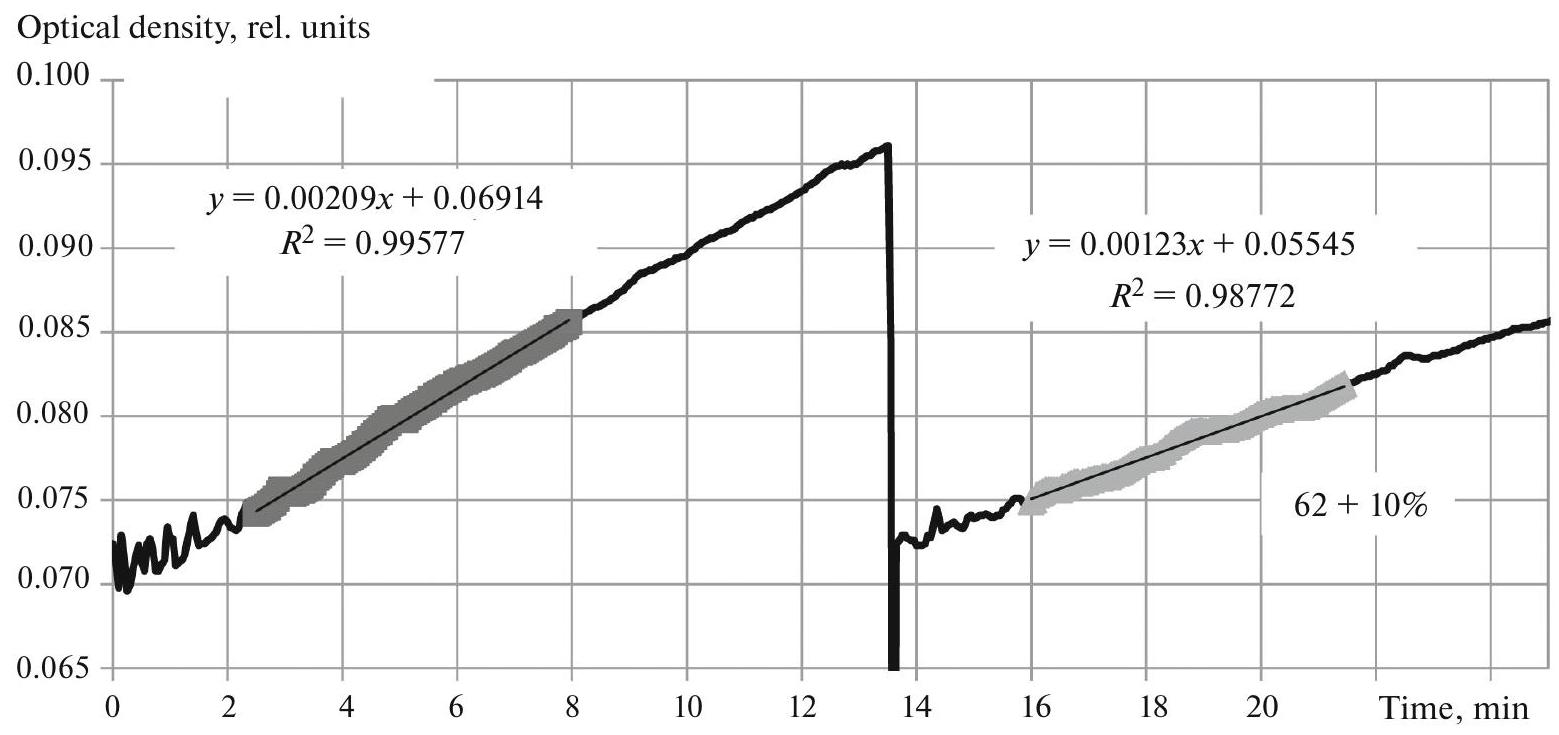
\includegraphics[scale=0.35, center]{2024_10_23_dfdc0589534473f41785g-8(1)}
Рис. 8. Влияние магнитного поля на активность иммобилизованного фермента для образца 8.\\
который был предложен нами ранее [25]. В случае этого механизма фермент должен быть одновременно присоединен («переприсоединен») к нескольким разным наночастицам. Тогда, в соответствии с данными, могут возникать силы в сотни пН, достаточные для изменения конформации и, следовательно, активности иммобилизованного фермента.
Таким образом, мы продемонстрировали возможность дистанционного управления биохимическими процессами за счет наномеханического воздействия на ферменты, иммобилизованные на магнитных наночастицах. Использование такого механизма воздействия открывает перспективы для различных медицинских приложений.\\
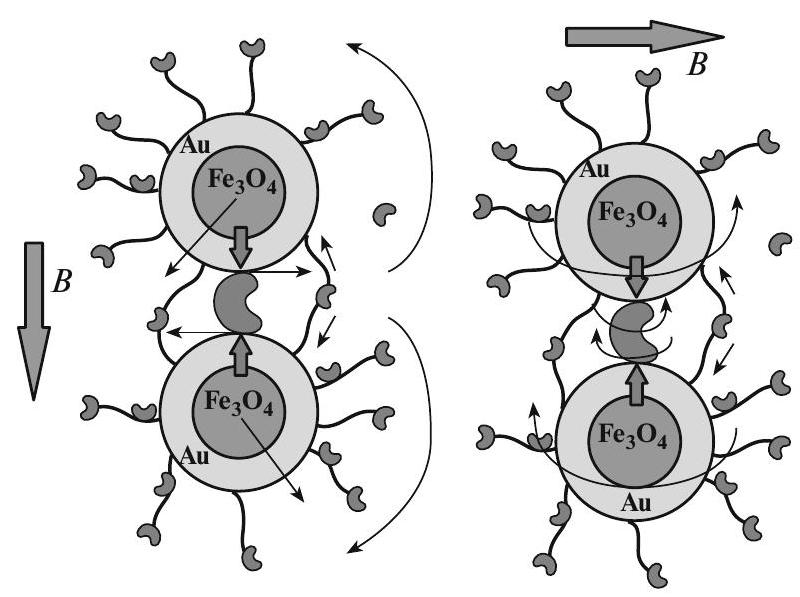
\includegraphics[scale=0.5, center]{2024_10_23_dfdc0589534473f41785g-8}
Рис. 9. Схема дистанционного наномеханического воздействия внешним магнитным полем на иммобилизованные биомолекулы.

\section*{ВЫВОДЫ}
В ходе данной работы были синтезированы и очищены наночастицы магнетит-золота с ядром-оболочкой размером \(23 \pm 3 \text{нм}\). Наночастицы были функционализированы бифункциональной липоевой кислотой благодаря ковалентному связыванию серы с поверхностью золота. Изучено влияние соотношения липоевая кислота/ПЭГ на коллоидную стабильность полученных наночастиц; установлено, что оптимальное соотношение липоевая кислота/ПЭГ составляет \(1: 16\). Наночастицы магнетит-золото были ковалентно функционализированы модельным ферментом химотрипсином, и была продемонстрирована возможность дистанционного управления работой фермента, иммобилизованного на магнитных наночастицах, с помощью переменного низкочастотного магнитного поля. Полученные нами наночастицы перспективны для использования в биомедицине и фармакологии.

\section*{СОЕДИНЕНИЯ}

\begin{figure*}[ht!]
  \centering
  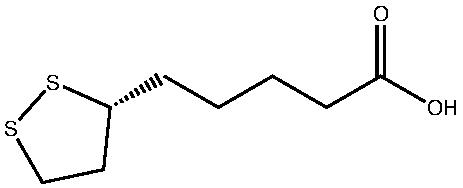
\includegraphics[scale=1]{lipoic.pdf}
  \captionsetup{labelformat=empty}
  \caption{5-(1,2-Дитиолиан-3ил)пентановая кислота (Липоевая Кислота)}
\end{figure*}

\begin{figure*}[ht!]
  \centering
  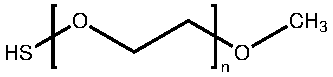
\includegraphics[scale=1]{hspegoch.pdf}
  \captionsetup{labelformat=empty}
  \caption{Меркапто-Метокси полиэтиленгликоль}
\end{figure*}

\begin{figure*}[ht!]
  \centering 
  \chemfig{H_3C--[1]N=C=N-[1]--[1]-N(-[1]CH_3)(-[5]CH_3)}
  \captionsetup{labelformat=empty}
  \caption{1-Этил-3-(3-диметиламинопроаил)карбодиимид}
\end{figure*}

\begin{figure*}[ht!]
  \centering 
  \chemfig{*5(-(=O)-N(-OH)-(=O)--)}
  \captionsetup{labelformat=empty}
  \caption{N-Гидроксисукцинимид}
\end{figure*}

\newpage

\section*{ЛИТЕРАТУРА}
0. Rudakovskaya, P.G., Lebedev, D.N., Efremova, M.V. et al. Сore–shell magnetite–gold nanoparticles: Preparing and functionalization by chymotrypsin. \\
Nanotechnolgies in Russia 11, 144–152 (2016). https://doi.org/10.1134/S1995078016020166
\begin{enumerate}
  \item R. Hergt, S. Dutz, R. Müller, et al., "Magnetic particle hyperthermia: nanoparticle magnetism and materials development for cancer therapy," J. Phys.: Condens. Matter 18, 2919-2934 (2006).
  \item K. J. Widder, A. E. Senyei, and D. G. Scarpelli, "Magnetic microspheres:a model system for site specific drug delivery in vivo," Proc. Soc. Exp. Biol. Med. 58, 141146 (1978).
  \item Y. J. Wang, "Superparamagnetic iron oxide based MRI contrast agents: Current status of clinical application," Quant. Imag. Med. Surg. 1, 36-40 (2011).
  \item C. Xu and S. Sun, "New forms of superparamagnetic nanoparticles for biomedical applications," Adv. Drug Deliv. Rev. 65, 732-743 (2013).
  \item F. Hasany, H. Abdurahman, R. Sunarti, and R. Jose, "Magnetic iron oxide nanoparticles: chemical synthesis and applications review," Curr. Nanosci. 9, 561-575 (2013).
  \item A. M. Derfus, G. Maltzahn, T. J. Harris, et al., "Remotely triggered release from magnetic nanoparticles," \\
  Adv. Mater. 19, 3932-3936 (2007).
  \item J. Chomoucka, J. Drbohlavova, D. Huska, V. Adamb, and J. Hubalek, "Magnetic nanoparticles and targeted drug delivering," Pharm. Res. 62, 144-149 (2010).
  \item T. K. Nguyen Thanh, Magnetic Nanoparticles: From Fabrication to Clinical Applications (CRC, Taylor and Francis, Boca Raton, London, New York, 2012).
  \item P. Majewski and B. Thierry, "Functionalized magnetite nanoparticles-synthesis, properties, and bioapplications," Crit. Rev. Solid State Mater. Sci. 32, 203-215 (2007).
  \item M. C. Daniel and D. Astruc, "Gold nanoparticles: assembly, supramolecular chemistry, quantum-sizerelated properties, and applications toward biology, catalysis, and nanotechnology," Chem. Rev. 104, 293346 (2004).
  \item P. G. Rudakovskaya, E. K. Beloglazkina, A. G. Mazhuga, N. L. Klyachko, A. V. Kabanov, N. V. Zyk, "Synthesis of magnetite-gold nanoparticles with core-shell structure," Vestn. Mosk. Univ., Ser. Khim. 56, 181-189 (2001).
  \item X. Zhao, Y. Cai, T. Wang, et al., "Preparation of alkan-ethiolate-functionalized core/shell \(\mathrm{Fe}_{3} \mathrm{O}_{4}-\mathrm{Au}\) nanoparticles and its interaction with several typical target molecules," Anal. Chem. 80, 9091-9096 (2008).
  \item U. Tamer, Y. Gündoğdu, I. HakkıBoyacı, et al., "Synthesis of magnetic core-shell \(\mathrm{Fe}_{3} \mathrm{O}_{4}-\mathrm{Au}\) nanoparticle for biomolecule immobilization and detection," J. Nanopart. Res. 12, 1187-1196 (2009).
  \item T. Ahmad, H. Bae, I. Rhee, et al., "Gold-coated iron oxide nanoparticles as a T2 contrast agent in magnetic resonance imaging," J. Nanosci. Nanotechnol. 12, 5132-5137 (2012).
  \item Ch. K. Lo, D. Xiao, and M. F. Choi, "Homocysteineprotected gold-coated magnetic nanoparticles: synthesis and characterization," J. Mater. Chem. 17, 24182427 (2007).
  \item P. G. Rudakovskaya, E. K. Beloglazkina, A. G. Majouga, and N. V. Zyk, "Synthesis and characterization of ter-pyridine-type ligand-protected gold-coated \(\mathrm{Fe}_{3} \mathrm{O}_{4}\) nanoparticles," \\
  Mendeleev Commun. 20, 158-160 (2010).
  \item A. Majouga, M. Sokolsky-Papkov, A. Kuznetsov, D. Lebedev, M. Efremova, E. Beloglazkina, P. Rudakovskaya, M. Veselov, N. Zyk, Y. Golovin, N. Klyachko, and A. Kabanov, "Enzyme-functionalized goldcoated magnetite nanoparticles as novel hybrid nanomaterials: synthesis, purification and control of enzyme function by low-frequency magnetic field," \\
  Colloids Surf. B: Biointerfaces 125, 104-109 (2015).
  \item N. L. Klyachko, M. Sokolsky-Papkov, N. Pothayee, M. V. Efremova, D. A. Gulin, A. A. Kuznetsov, A. G. Majouga, J. S. Riffle, Y. I. Golovin, and A. V. Kabanov, "Changing the enzyme reaction rate in magnetic nanosuspensions by a non-heating magnetic field," Angew. Chem. Int. Ed. Engl. 51, 12016 (2012).
  \item T. Ahmad, H. Bae, I. Rhee, et al., "Gold-coated iron oxide nanoparticles as a T2 contrast agent in magnetic resonance imaging," J. Nanosci. Nanotechnol. 12, 5132-5137 (2012).
  \item Yu-Hui Bai, Jin-Yi Li, Jing-Juan Xu, and Hong-Yuan Chena, "Ultrasensitive electrochemical detection of DNA hybridization using \(\mathrm{Au} / \mathrm{Fe}_{3} \mathrm{O}_{4}\) magnetic composites combined with silver enhancement," \\
  Affiliat. Analyst 135, 1672-1679 (2010).
  \item I. Robinson, D. Tung, S. Maenosono, et al., "Synthesis of core-shell gold coated magnetic nanoparticles and their interaction with thiolated DNA," \\
  Nanoscale 12, 2624-2630 (2010).
  \item W. Qian, M. Murakami, Y. Ichikawa, and Y. Che, "Highly efficient and controllable PEGylation of gold nanoparticles prepared by femtosecond laser ablation in water," J. Phys. Chem. C 115, 23293-23298 (2011).
  \item J. Vidal-Vidal, J. Rivasb, M. A. López-Quintela, "Synthesis of monodisperse maghemite nanoparticles by the microemulsion method," \\
  ColloidSurf. A: Physicochem. Eng. Asp. 288, 44-51 (2006).
  \item W. Appel, "Chymotrypsin: molecular and catalytic properties," Clin. Biochem. 19, 317-322 (1986).
  \item Yu. I. Golovin, N. L. Klyachko, D. Yu. Golovin, M. V. Efremova, A. A. Samodurov, M. Sokolski-Papkov, and A. V. Kabanov, "A new approach to the control of biochemical reactions in a magnetic nanosuspension using a low-frequency magnetic field," Tech. Phys. Lett. 39, 240 (2013).
  \item J. C. Phillips, K. Schulten, et al., "Scalable molecular dynamics with NAMD," J. Comput. Chem. 26, 17811802 (2005).
\end{enumerate}

\end{document}